\section{Results}

\subsection{Permeability in Poiseuille flow}
We will go back to the Poiseuille flow described in section \ref{sec:dsmc_validation_poiseuille}; two infinite parallel plates with temperature $T$ and an applied acceleration in the $z$-direction, see figure \ref{fig:dsmc_poiseuille_system}. 

\begin{figure}[htp]
\centering
%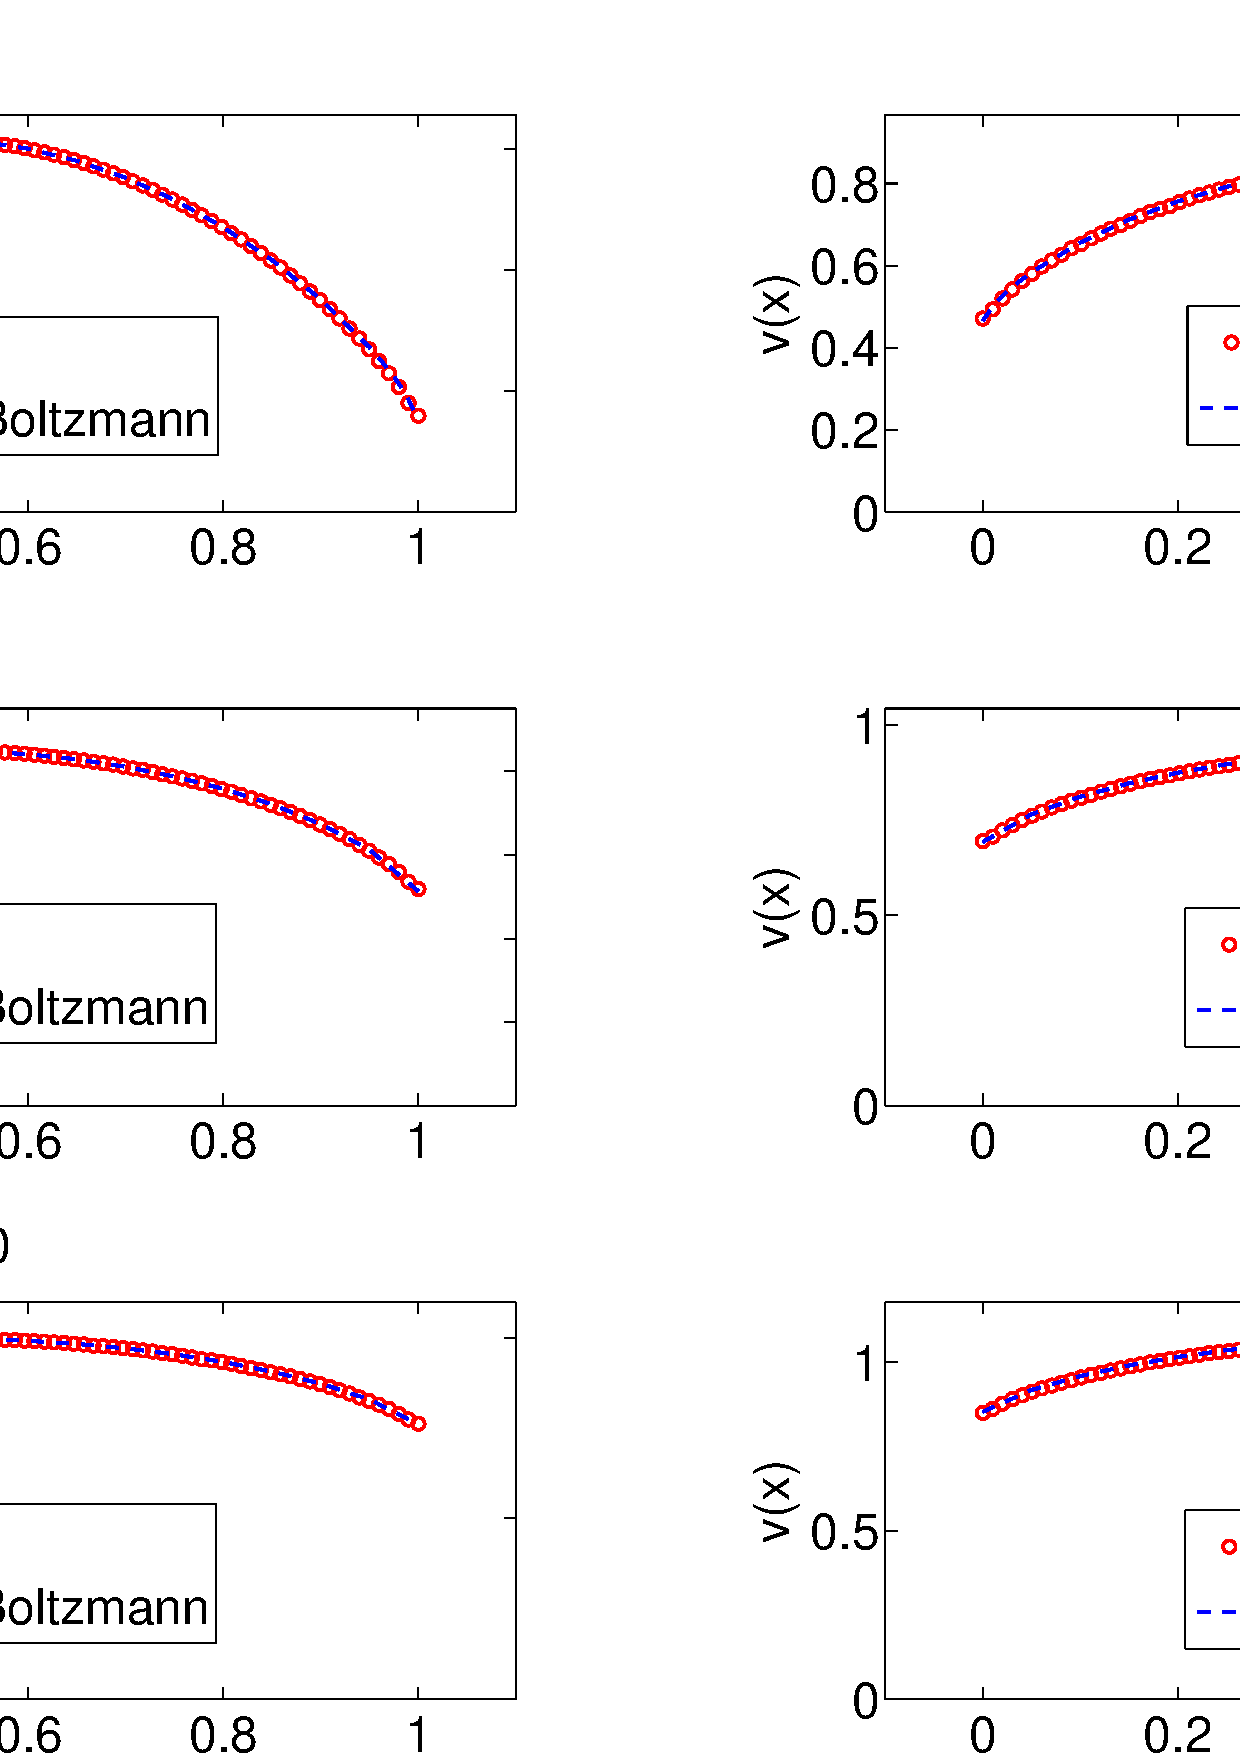
\includegraphics[scale=0.25]{figures/validation_poiseuille.pdf}
\label{fig:dsmc_poiseuille_system}
\caption{Acceleration driven Poiseuille flow}
\end{figure}

\subsection{Cylinders}

\subsection{Randomly packed spheres}
Through the Carman-Kozeny equation, we can theoretically predict the permeability for randomly packed spheres 
\begin{align}
	k = {a^2 \over 9K} {\phi^3 \over (1 - \phi)^2},
\end{align}
where $\phi$ is the porosity, $a$ is the sphere radius and $K$ Kozeny constant which is experimentally measured to be around five\cite{carman1937fluid}. This theoretical result has been verified to predict permeabilities in experiments, but at micrometer scale, we expect deviations. 

\subsection{Random walk}
We can create a geometry with a statistical interesting structure. If we start with a completely filled volume, we can release $N$ random walkers at different start locations, and let them carve out tunnels of which the particles can be in. 
\subsection{Sprekknettverk}
